% !TeX spellcheck = en_US
\documentclass[letterpaper,12pt,twoside]{report}
\usepackage{fancyhdr}
\usepackage{fullpage}
\usepackage{tikz}
\usepackage{amsmath}

\begin{document}
	\pagestyle{fancy}
	\fancyhf{}
	\fancyhead[L]{Day 18}
	\fancyhead[R]{\textit{The Calendar Project}}
	\fancyfoot[L]{Citations Involved: none}
	
	% Problem
	\paragraph{Problem}
	\begin{quote}
		\textsf{A block of wood in the shape of a right rectangular prism has dimensions $1 \textrm{ft} \times 1 \textrm{ft} \times 2 \textrm{ft}$. If Vasu saws it in half to create two triangular prisms with height $1 \textrm{ft}$, what is the percentage increase in total surface area?}
	\end{quote}
	
	% Graphics
	\begin{center}
		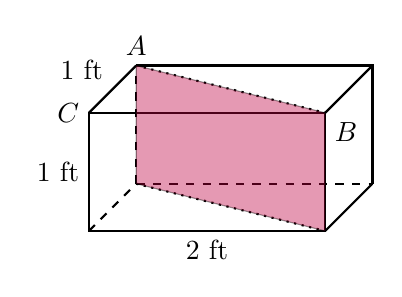
\begin{tikzpicture}[scale=1.5]
		\draw[thick] (0,0) -- (0,1) -- (2,1) -- (2,0) -- cycle;
		\draw[thick] (2.4,0.4) -- (2.4,1.4) -- (0.4,1.4);
		\draw[thick][dashed] (0.4,0.4) -- (0.4,1.4);
		\draw[thick][dashed] (0,0) -- (0.4,0.4);
		\draw[thick][dashed] (0.4,0.4) -- (2.4,0.4);
		\draw[thick] (0,1) -- (0.4,1.4);
		\draw[thick] (2,1) -- (2.4,1.4);
		\draw[thick] (2,0) -- (2.4,0.4);
		
		\draw[thick][dotted] (0.4,1.4) -- (2,1);
		\draw[thick][dotted] (0.4,0.4) -- (2,0);
		\draw[fill=purple][opacity=0.4] (0.4,1.4) -- (0.4,0.4) -- (2,0) -- (2,1) -- cycle;
		
		\node[below] at (1,0) {$2$ ft};
		\node[left] at (0,0.5) {$1$ ft};
		\node[above left] at (0.2,1.2) {$1$ ft};
		
		\node[above] at (0.4,1.4) {$A$};
		\node[below right] at (2,1) {$B$};
		\node[left] at (0,1) {$C$};
		
		\end{tikzpicture}
	\end{center}
	
	% Reasoning
	\paragraph{Reasoning}
	\begin{quotation}
		
		The formula for surface area for prisms is $LA+2B$ where $LA=hp$ (4).
		
		The perimeter of the rectangular prism's base is $p=2(1+2)=6 \text{ft}$; its area is $bh=2\times 1=2 \text{ft}^2$ (3). The rectangular prism's lateral area is $hp=(1)(6)=6 \text{ft}^2$ (3); its surface area is $6+2(2)=10 \text{ft}^2$.
		
		$AB$, according to the Pythagorean Theorem ($a^2+b^2=c^2$) (1), is $\sqrt{1^2+2^2}=\sqrt{5}$. Since $\overline{AB}$ is the hypotenuse of $\triangle ABC$ (the base for each triangular prism), the perimeter of each triangular prism's base is $1+2+\sqrt{5}=3+\sqrt{5}$; its area is $\frac{1}{2}bh=\frac{1}{2}(2)(1)=1 \text{ft}^2$ (2). The lateral area of each triangular prism is $hp=1(3+\sqrt{5})=(3+\sqrt{5}) \text{ft}^2$ (3); its surface area is $(3+\sqrt{5})+2(1)=(5+\sqrt{5}) \text{ft}^2$.
		
		The percentage increase in total surface area can be represented as $\frac{2(5+\sqrt{5})-10}{10}$ because the rectangular prism was cut into \textbf{two} congruent triangular prisms. This is simplified and evaluated as follows:
		
		\begin{center}
			\begin{tabular}{l | l}
				$\frac{10+2\sqrt{5}-10}{10}$ & Apply the Distributive Property \\
				$\frac{2\sqrt{5}}{10}$ & Simplify the numerator \\
				$\frac{\sqrt{5}}{5}$ & Simplify the fraction \\
				$\approx 0.4472$ & Evaluate the expression
			\end{tabular}		
		\end{center}
	
	The solution to this problem is therefore $\boxed{\approx 44.72\%}$.
	\end{quotation}
	
	\paragraph{External References}
	
	\begin{enumerate}
		\item Textbook Ch. 9, Pg. 587: Pythagorean Theorem (Theorem 1-6-1)
		\item Textbook Ch. 9, Pg. 590: Area of Triangles and Trapezoids
		\item Textbook Ch. 9, Pg. 589: Area of Parallelograms
		\item Textbook Ch. 10, Pg. 680: Lateral Area and Surface Area of Right Prisms
	\end{enumerate}
	
\end{document}